\chapter{Alternative Systemer}
\label{Comparison}
Udover at udvikle vores udgave af et booking-system til IT-Universitetet, vil vi i dette kapitel give en kort beskrivelse af to alternative  systemer og sammenligne dem med vores løsning.

\section{Room Booking System}
\label{Comparison_RBS}
"Room Booking System"\footnote{http://www.roombookingsystem.co.uk/} er et web-baseret booking system designet til at opfylde både skoler og virksomheders behov. 

Interfacet er designet som en kalender, hvor man kan vælge hvilke kategorier af ressourcer man kan vil se tider for eksempelvis, IT rum, mødelokaler, projekter eller andet udstyr. Bookinger af diverse ressourcer er ligesom vores system opgjort i farvekoder så man hurtigt kan få et overblik over hvad der er ledigt og hvad der er booket. Figur \ref{Comparison_RBS_RoomBookingSystem} visser det først skærmbillede i "Room Booking System"

\begin{figure}[h!]
  \centering
    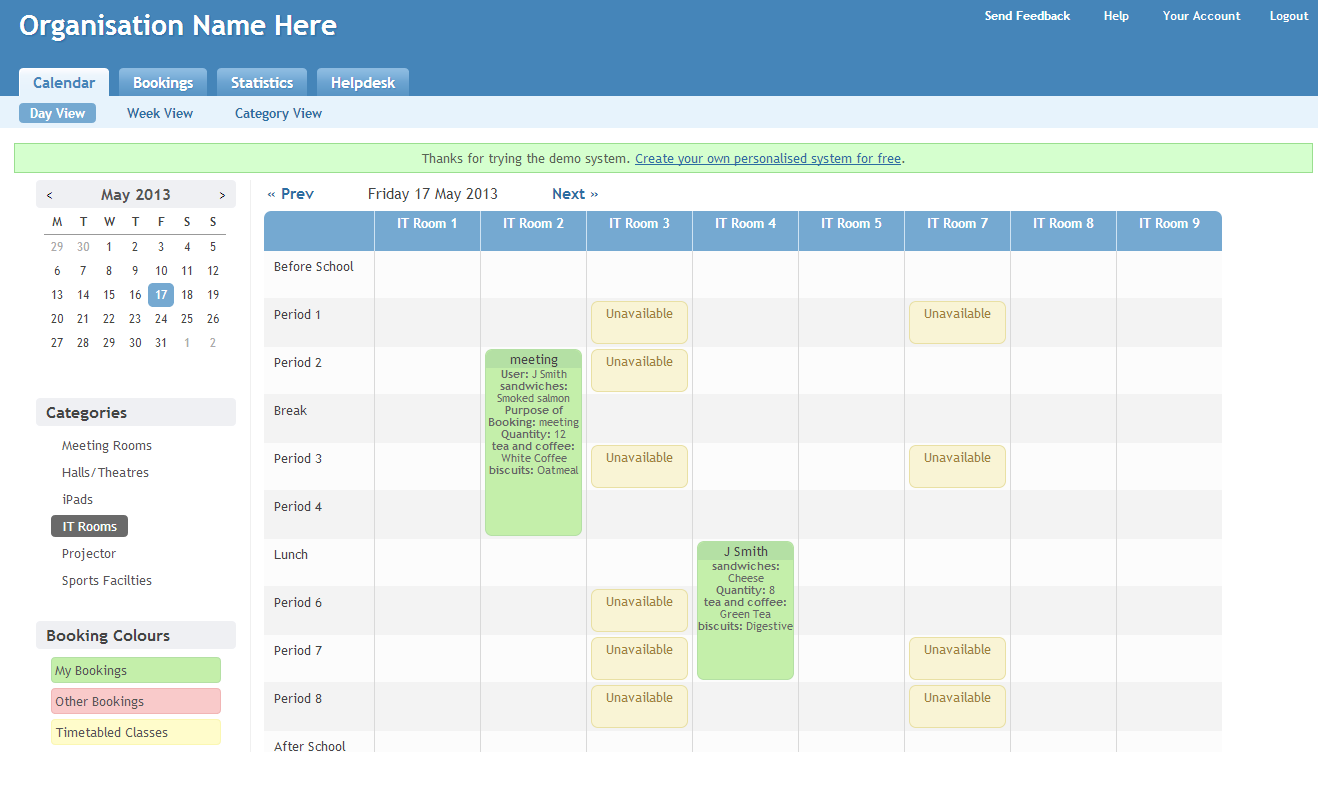
\includegraphics[width=0.8\textwidth]{Appendix/GUI-Prototype/RoomBookingSystem}
  \caption{Det først skærmbillede i systemet som visser oversigten over booket ressourcer}
\label{Comparison_RBS_RoomBookingSystem}
\end{figure}

"Room Booking System" giver også mulighed for tilføje forplejning til ens bookinger. Figur \ref{Comparison_RBS_RoomBookingSystemList} visser skærmbilledet der svare til vores booking-liste, her kan det ses at der til bookingen er blevet bestilt sandwicher med røget laks plus te og kiks.

\begin{figure}[h!]
  \centering
    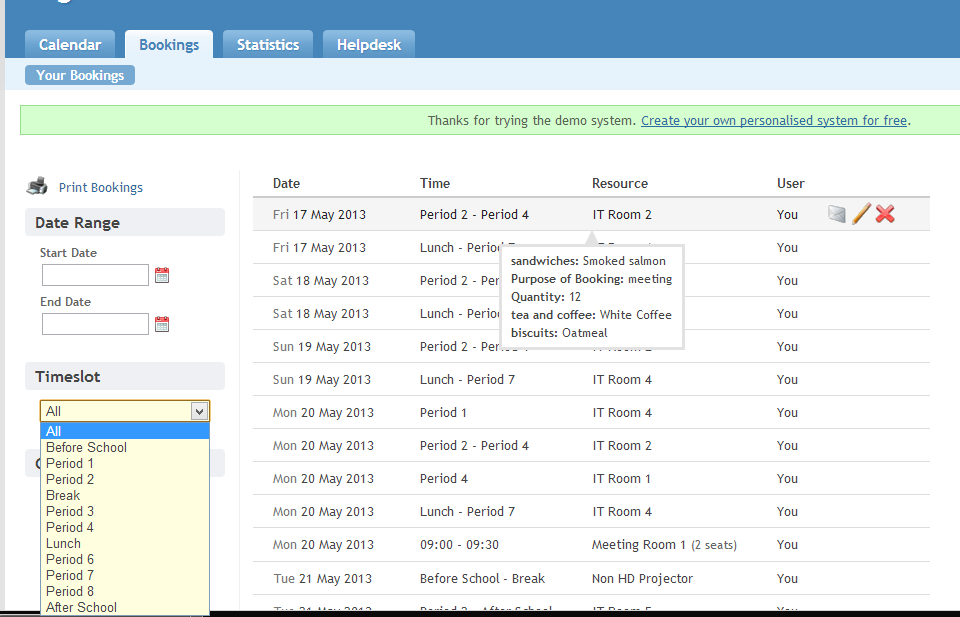
\includegraphics[width=0.8\textwidth]{Appendix/GUI-Prototype/RoomBookingSystemList}
  \caption{Skærmbillede over de bookinger der i systemet}
\label{Comparison_RBS_RoomBookingSystemList}
\end{figure}

Desuden er login til systemet seperat og dermed er der ikke mulighed for at integrere det med hverken Active Directory (AD) eller Where Are You From (WAYF). Et abonnement, der understøtter 200 lokaler/udstyr og 500 brugere, koster 434 kr. om måneden.

En fordel ved "Room Booking System" er, at det giver mulighed for at lave statistikker se figur \ref{Comparison_RBS_RoomBookingSystemStatistic}. Desuden kan det ses som en fordel, at det er hostet eksternt.

\begin{figure}[h!]
  \centering
    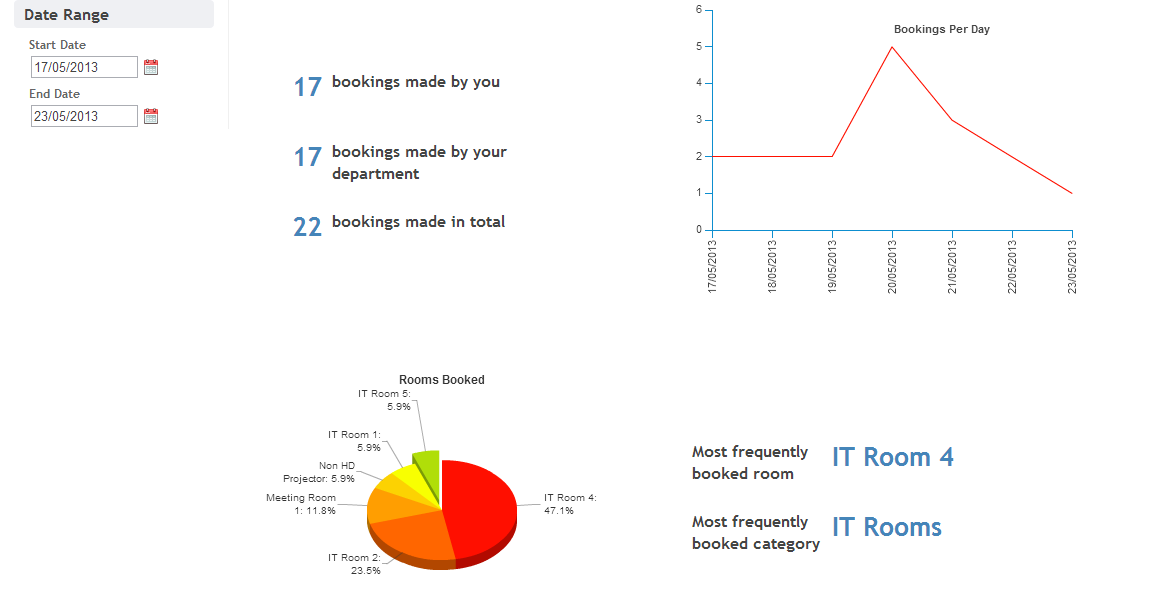
\includegraphics[width=0.8\textwidth]{Appendix/GUI-Prototype/RoomBookingSystemStatistic}
  \caption{Skærmbillede til visning af statestik over booking af ressourcer.}
\label{Comparison_RBS_RoomBookingSystemStatistic}
\end{figure}

Ulempen ved "Room Booking System" i forhold til vores løsning er, at der er en grænse for hvor mange lokaler og udstyrselementer, som kan bookes i systemet. Desuden er det ikke muligt at integrere med et eksisterende ITU login system. Da der kun er mulighed for 500 brugere i systemet, vil nogle brugere skulle slettes for, at der kan oprettes nye i forbindelse med nye studerende/ansatte.

Hvis man vil afprøve systemet er der i menubaren på hjemmesiden et punkt der hedder demo. Der kan man frit prøve og undersøge interfacet og dets feature uden at skulle oprette bruger eller downloade nogen klient.

\section{School Booking}
\label{Comparison_SB}
"School Booking"\footnote{http://www.schoolbooking.com/} er et andet web-baseret system, som primært er designet til brug af skoler. 

Systemet giver mulighed for at booke både lokaler og udstyr\footnote{Det bookede udstyr kan være forplejning, hvis man sætter rigtigt op.}. Man kan betale ekstra for at tillade eksterne bookere. Statetisk er også muligt i dette system. Der er dog ikke mulighed for at integrere det med AD eller WAYF.

Et system, der understøtter 1000 brugere, 300 lokaler/resurser, eksterne bookere og statestik koster årligt ~11.500 kr.

Fordelen ved dette system er det samme som ved "Room Booking System": muligheden for at lave statestik.

Ulempen ved dette system er, at der er en begrænset mængde af brugere, som kan anvende systemet, samt at det ikke er muligt at integrere det med AD eller lignende, fordi det er hostet eksternt.

Vi har desvære ingen mulighed for at undersøge brugervenligheden af systemet da der ikke var nogen offentlige screenshots og det krævede at man skulle være en registrer bruger for, at man kunne prøve deres 30 dags gratis prøveperiode.